\clearpage
\section{Effects from $\lcp$ excited states}
\label{app:lcst}

In this analysis, the single tag method is used to increase the statistics by reconstructing a single $\lcp$. There could be potential contributions from the decays of $\lcp$ excited states only at two high energy points $\sqrt{s} = 4.918$ and 4.950$\gev/c^2$, which are just above the production threshold of $\Lambda_c^{*+}\lcm$. The effects are expected to be negligible due to the $\Delta E$ requirements in the $\mbc$ signal region. The corrected recoil mass of $\lcp$ ($RQ(\lcp)$) is defined as
\begin{equation}
    RQ(\lcp) = RM(\lcp) + M(\lcp) - m_{\rm PDG}(\lcp),
\end{equation}
where $RM(\lcp)$ is the recoil mass of $\lcp$, $M(\lcp)$ is the invariant mass of $pK^-\pi^+$ and $m_{\rm PDG}(\lcp)$ is the nominal mass value of $\lcp$ in PDG. After all selections, the distribution of $RQ(\lcp)$ for data at $\sqrt{s} = 4.918\gev$ is shown in Figure~\ref{fig:data_rm_lmdc}. A clear peak is observed around the nominal mass value of $\lcp$ associated with a flat background contributions, which indicates that the selected events are mainly from the $\lcp\lcm$ process instead of excited $\lcp$ states.
\begin{figure}[H]\centering
    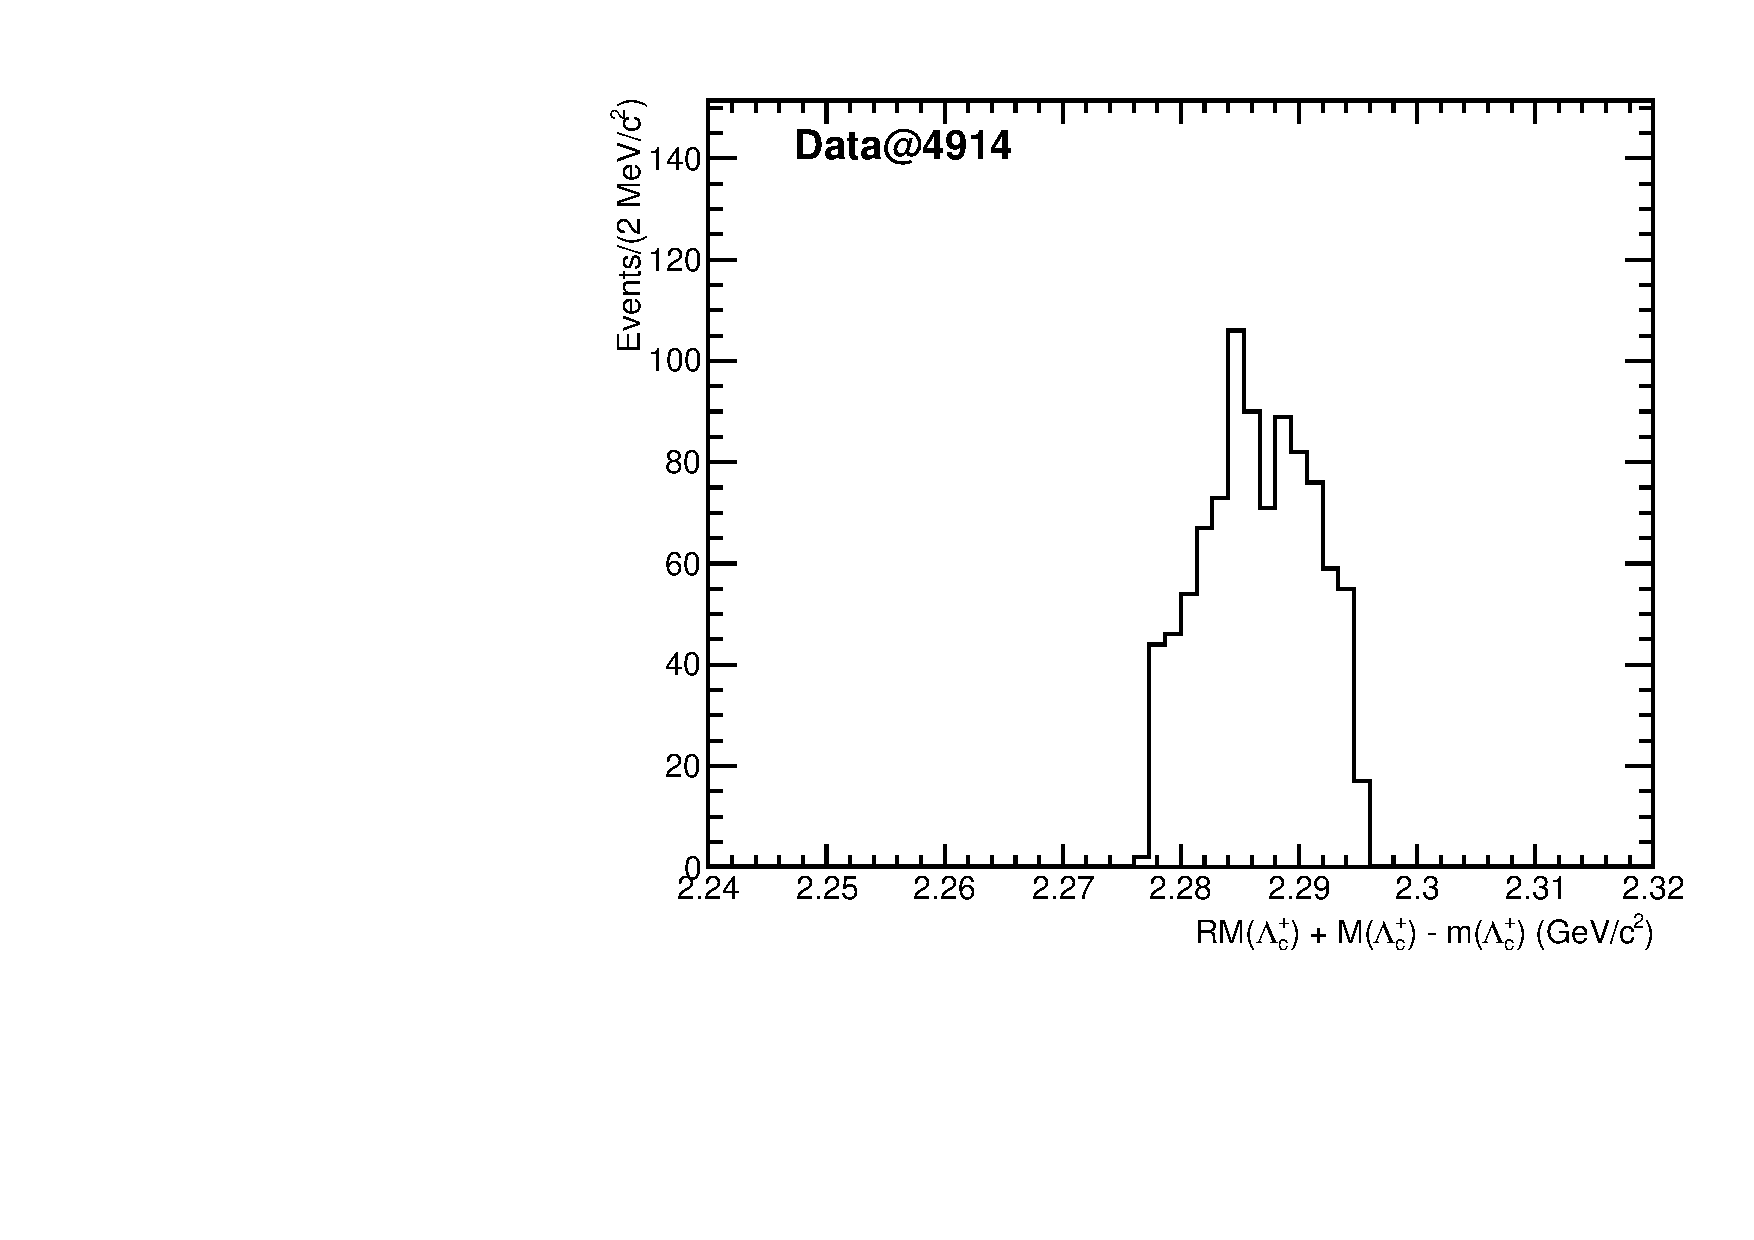
\includegraphics[width=0.45\textwidth]{figure/app_lcst/output_data_4914_rm_lmdc.pdf}
    \caption{Distribution of $RQ(\lcp)$ for data at $\sqrt{s} = 4.918\gev$.}
\label{fig:data_rm_lmdc}
\end{figure}

In order to estimate the contribution from the $\Lambda_c^{*+}\lcm$, two sets of MC samples are generated for $\Lambda_c(2595)^+$ and $\Lambda_c(2625)^+$ with 260k events. The associated $\lcm$ decays inclusively, the decays of $\Lambda_c^{*+}$ are listed below:
\begin{itemize}
    \item $\Lambda_c^{*+} \to \Sigma_c^{++}\pim$, $\Sigma_c^{++} \to \lcp\pip$, $\lcp \to pK^-\pip$.
    \item $\Lambda_c^{*+} \to \Sigma_c^{0}\pip$, $\Sigma_c^{0} \to \lcp\pim$, $\lcp \to pK^-\pip$.
    \item $\Lambda_c^{*+} \to \Sigma_c^{+}\piz$, $\Sigma_c^{+} \to \lcp\piz$, $\lcp \to pK^-\pip$.
    \item $\Lambda_c^{*+} \to \lcp\pip\pim$, $\lcp \to pK^-\pip$. 
    \item $\Lambda_c^{*+} \to \lcp\piz\piz$, $\lcp \to pK^-\pip$.
\end{itemize}
The fraction of each decay of $\Lambda_c^{*+}$ are set to be equal. The $\Delta E$ distributions are shown in Figure~\ref{fig:mc_lcst_deltaE}, which show a significant deviation to 0 for both $\Lambda_c^{*+}\lcm$ samples. After applying the $\Delta E$ requirements of (-0.029, 0.026)$\gev$, the $\mbc$ distributions are shown in Figure~\ref{fig:mc_lcst_mbc}. The distributions of $RQ(\lcp)$ are shown in Figure~\ref{fig:mc_lcst_rm_lmdc} in $\mbc$ signal region. There are 47 and 44 events remaining within $\mbc$ signal region of (2.282, 2.291)$\gev/c^2$ for $\Lambda_c(2595)^+\lcm$ and $\Lambda_c(2625)^+\lcm$, respectively. Both processes have very low selection efficiency less than 0.02\%. The production cross sections of $\Lambda_c^{*+}\lcm$ are measured by BAM-627, the total number of $\Lambda_c^{*+}\lcm$ are calculated and listed in Table~\ref{tab:total_lcst}. Considering the $\BR(\lcm \to \bar{p}K^+\pi^-) = 6.26\%$, $\BR(\Lambda_c^{*+} \to \lcp\pi\pi) = 1$ and selection efficiency, the survive $\Lambda_c^{*+}\lcm$ events after our selections will be less than 0.2. In conclusion, the contributions from excited $\lcp$ states are negligible.

%Considering the production cross sections of $\Lambda_c^{*+}\lcm$, the containments of $\lcp$ excited states are negligible.

\begin{figure}[H]\centering
    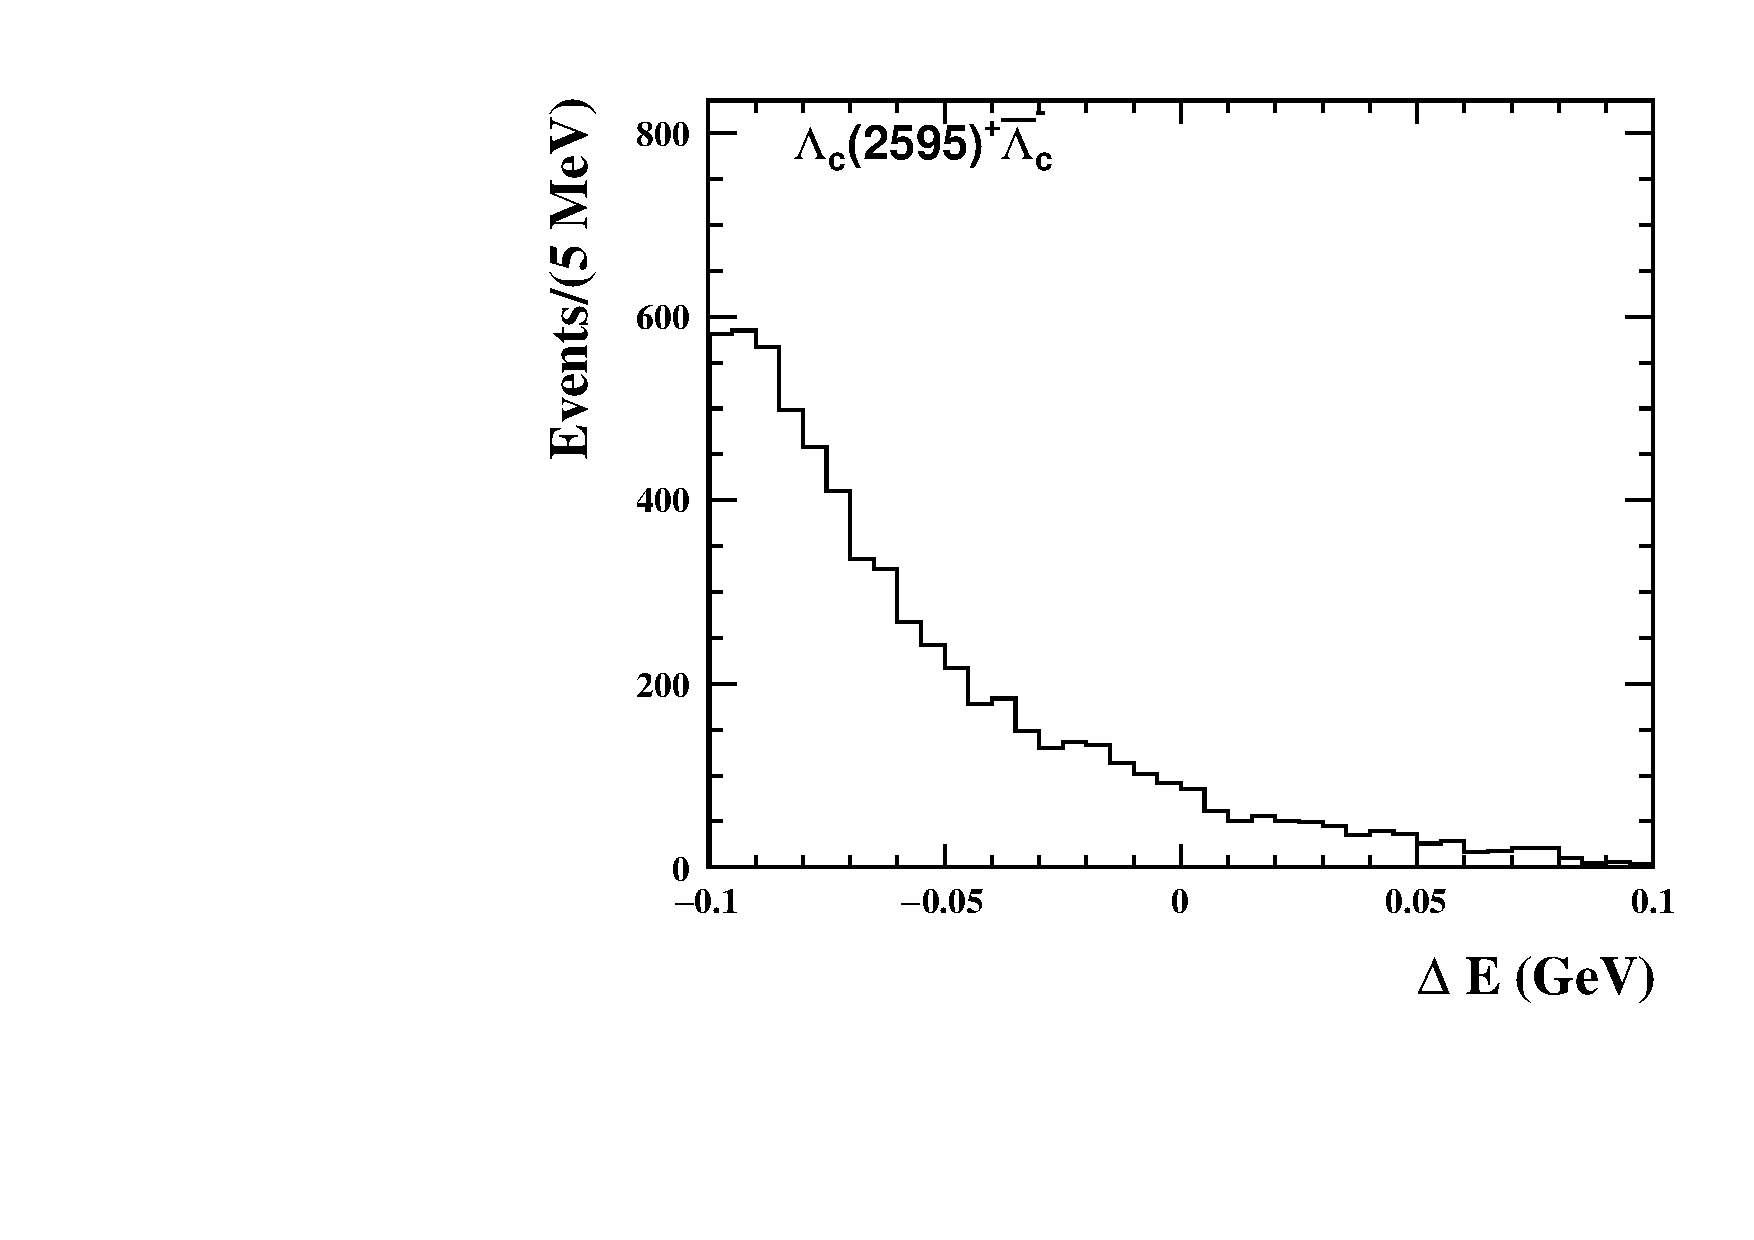
\includegraphics[width=0.45\textwidth]{figure/app_lcst/output_Lc2595_4914_deltaE.pdf}
    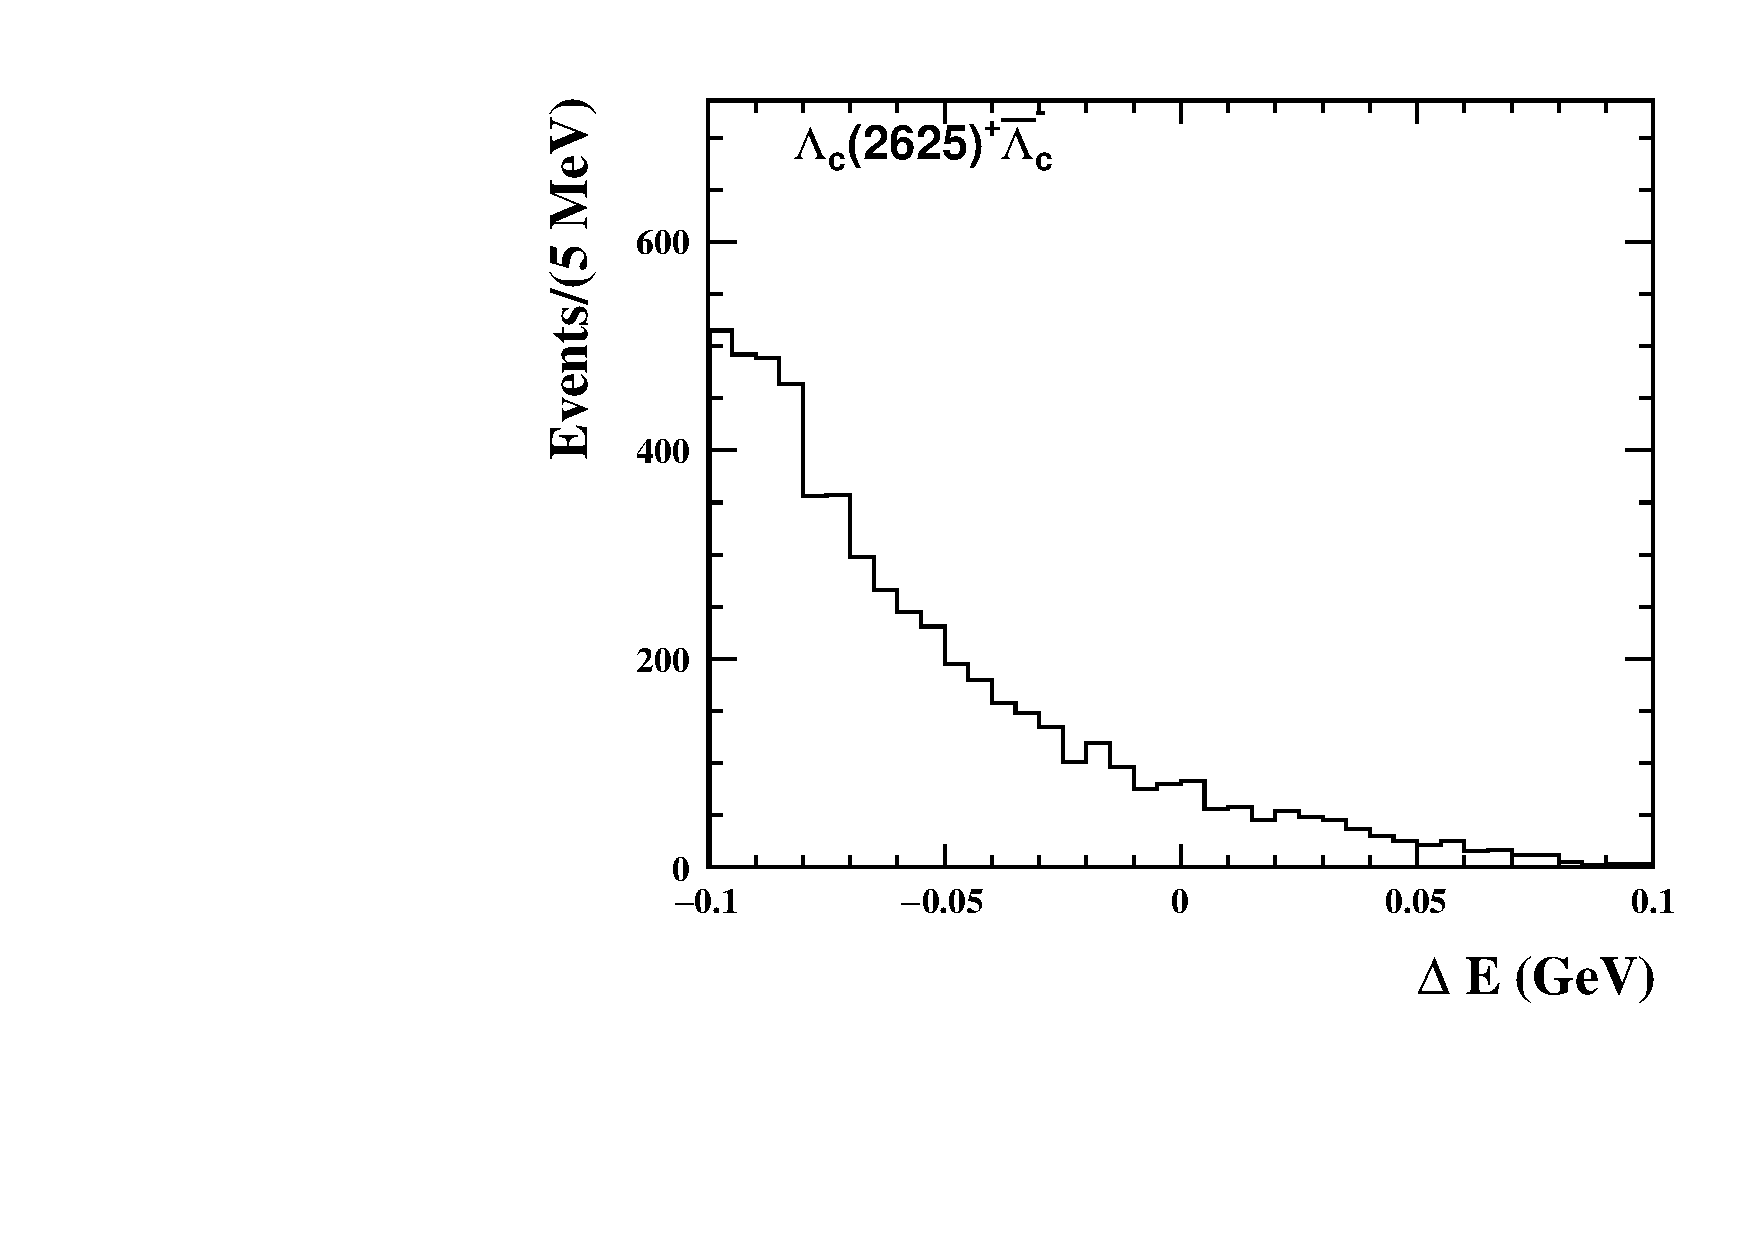
\includegraphics[width=0.45\textwidth]{figure/app_lcst/output_Lc2625_4914_deltaE.pdf}
    \caption{Distribution of $\Delta E$ for  $\Lambda_c(2595)^+\lcm$ (left) and $\Lambda_c(2625)^+\lcm$ (right) at $\sqrt{s} = 4.918\gev$.}
\label{fig:mc_lcst_deltaE}
\end{figure}

\begin{figure}[H]\centering
    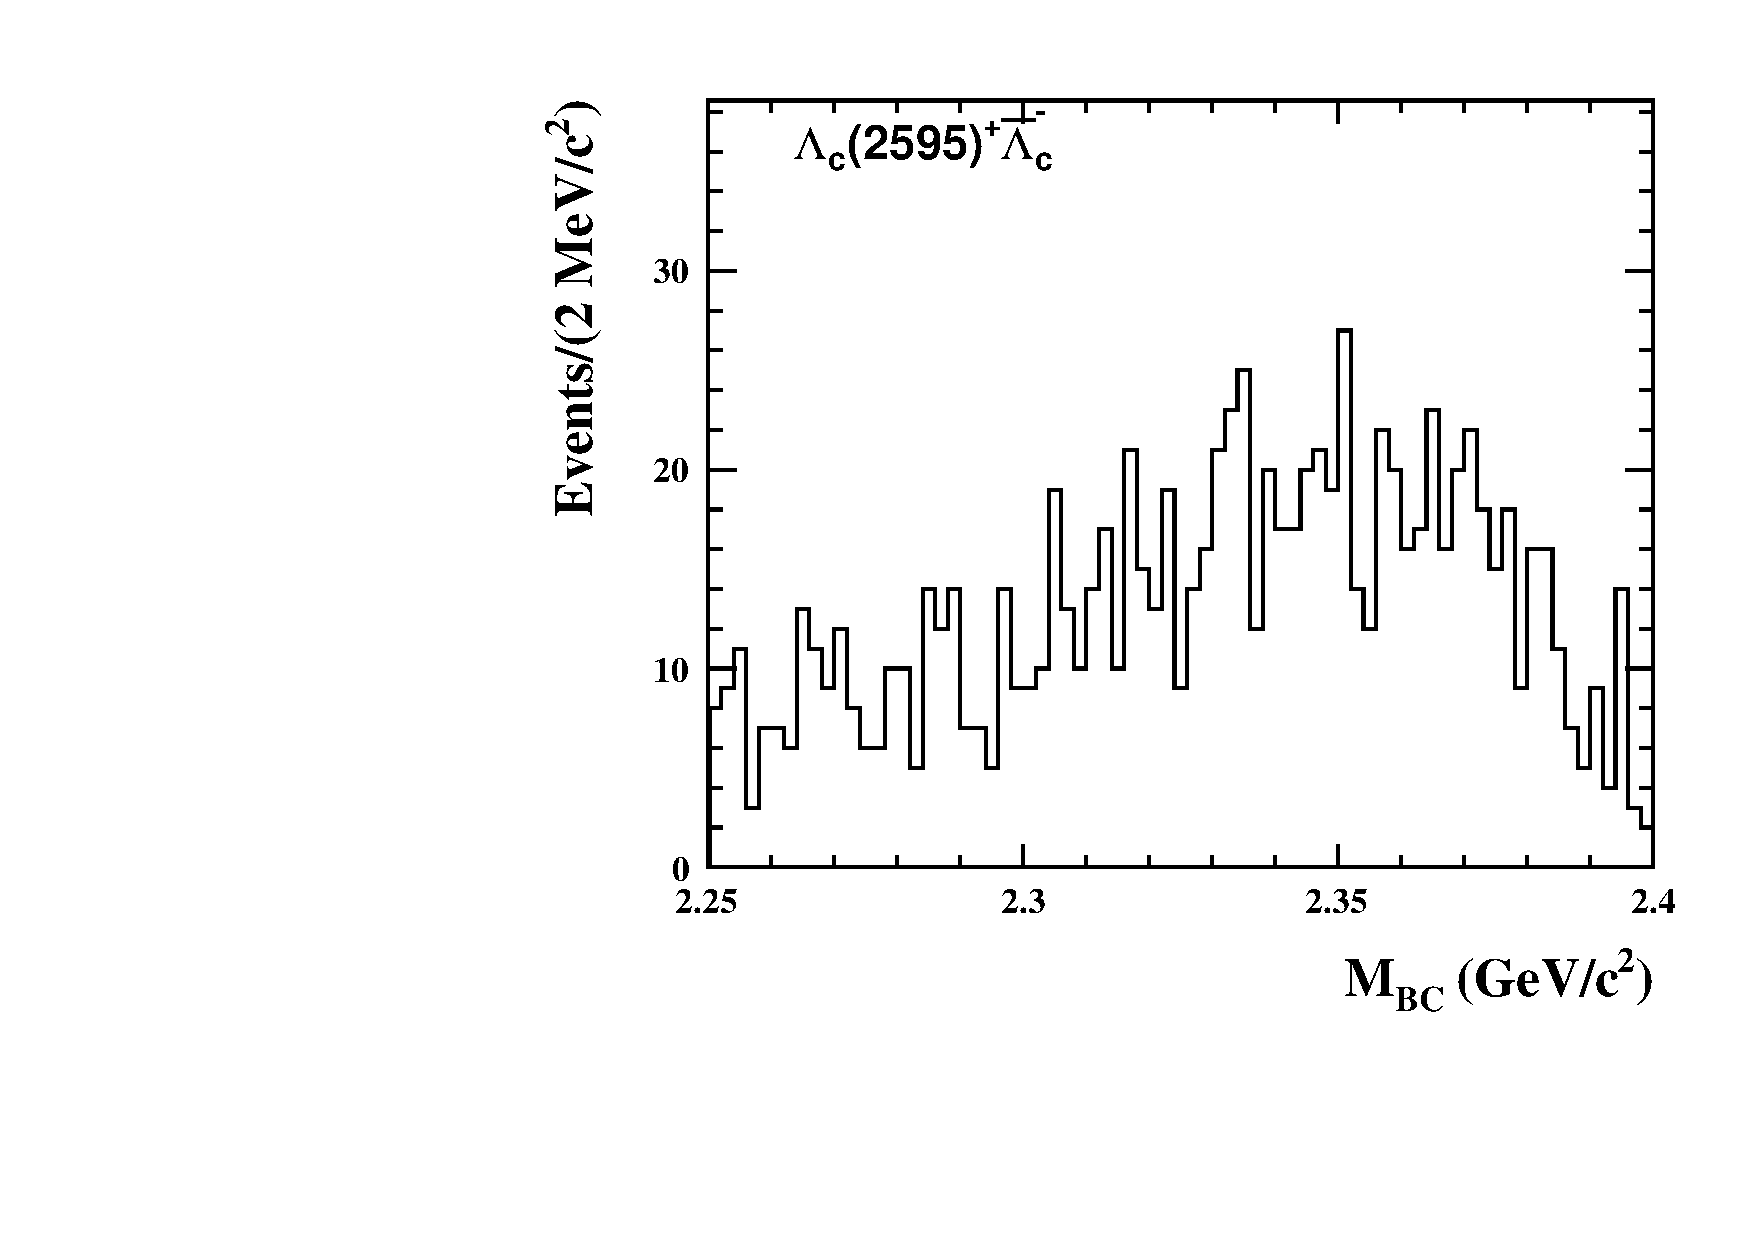
\includegraphics[width=0.45\textwidth]{figure/app_lcst/output_Lc2595_4914_mBC.pdf}
    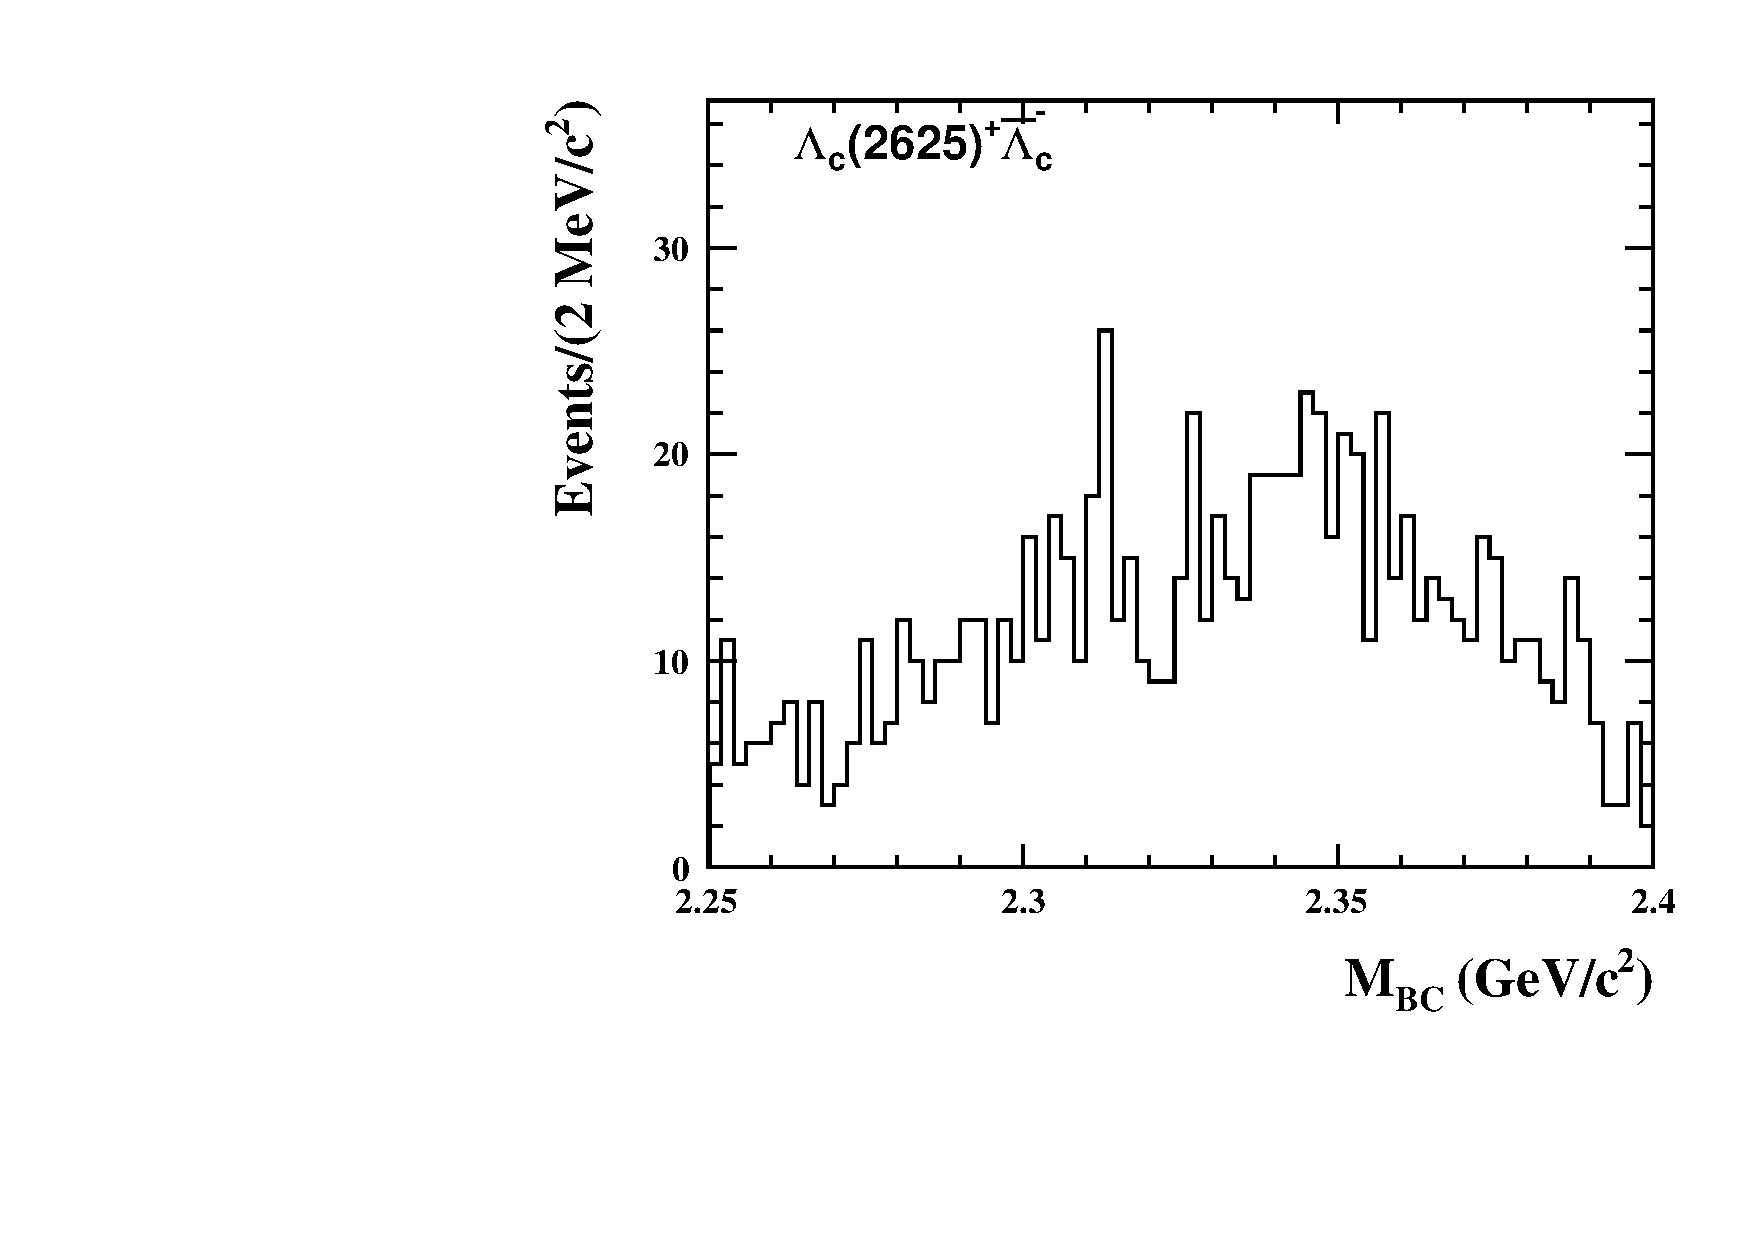
\includegraphics[width=0.45\textwidth]{figure/app_lcst/output_Lc2625_4914_mBC.pdf}
    \caption{Distribution of $\mbc$ for  $\Lambda_c(2595)^+\lcm$ (left) and $\Lambda_c(2625)^+\lcm$ (right) at $\sqrt{s} = 4.918\gev$ after $\Delta E$ requirements applied.}
\label{fig:mc_lcst_mbc}
\end{figure}

\begin{figure}[H]\centering
    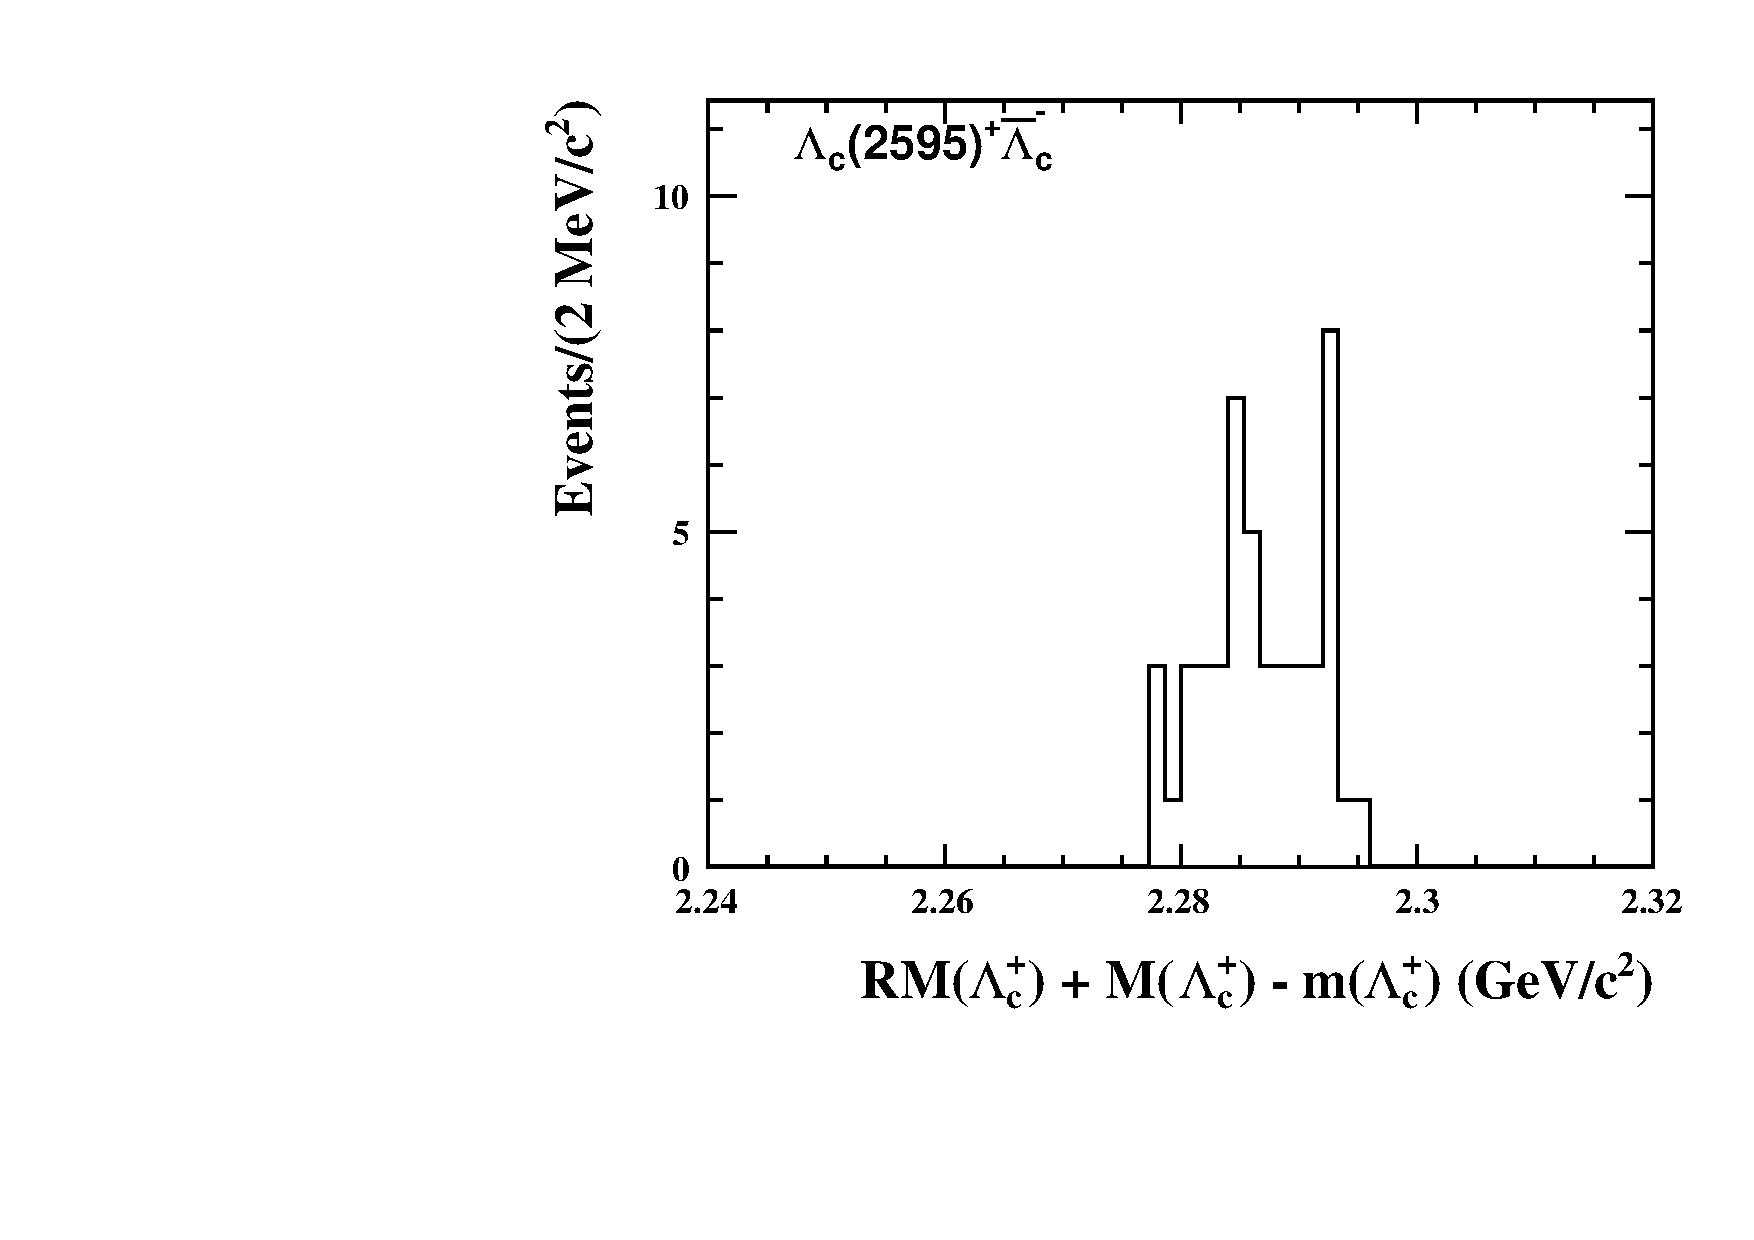
\includegraphics[width=0.45\textwidth]{figure/app_lcst/output_Lc2595_4914_rm_lmdc.pdf}
    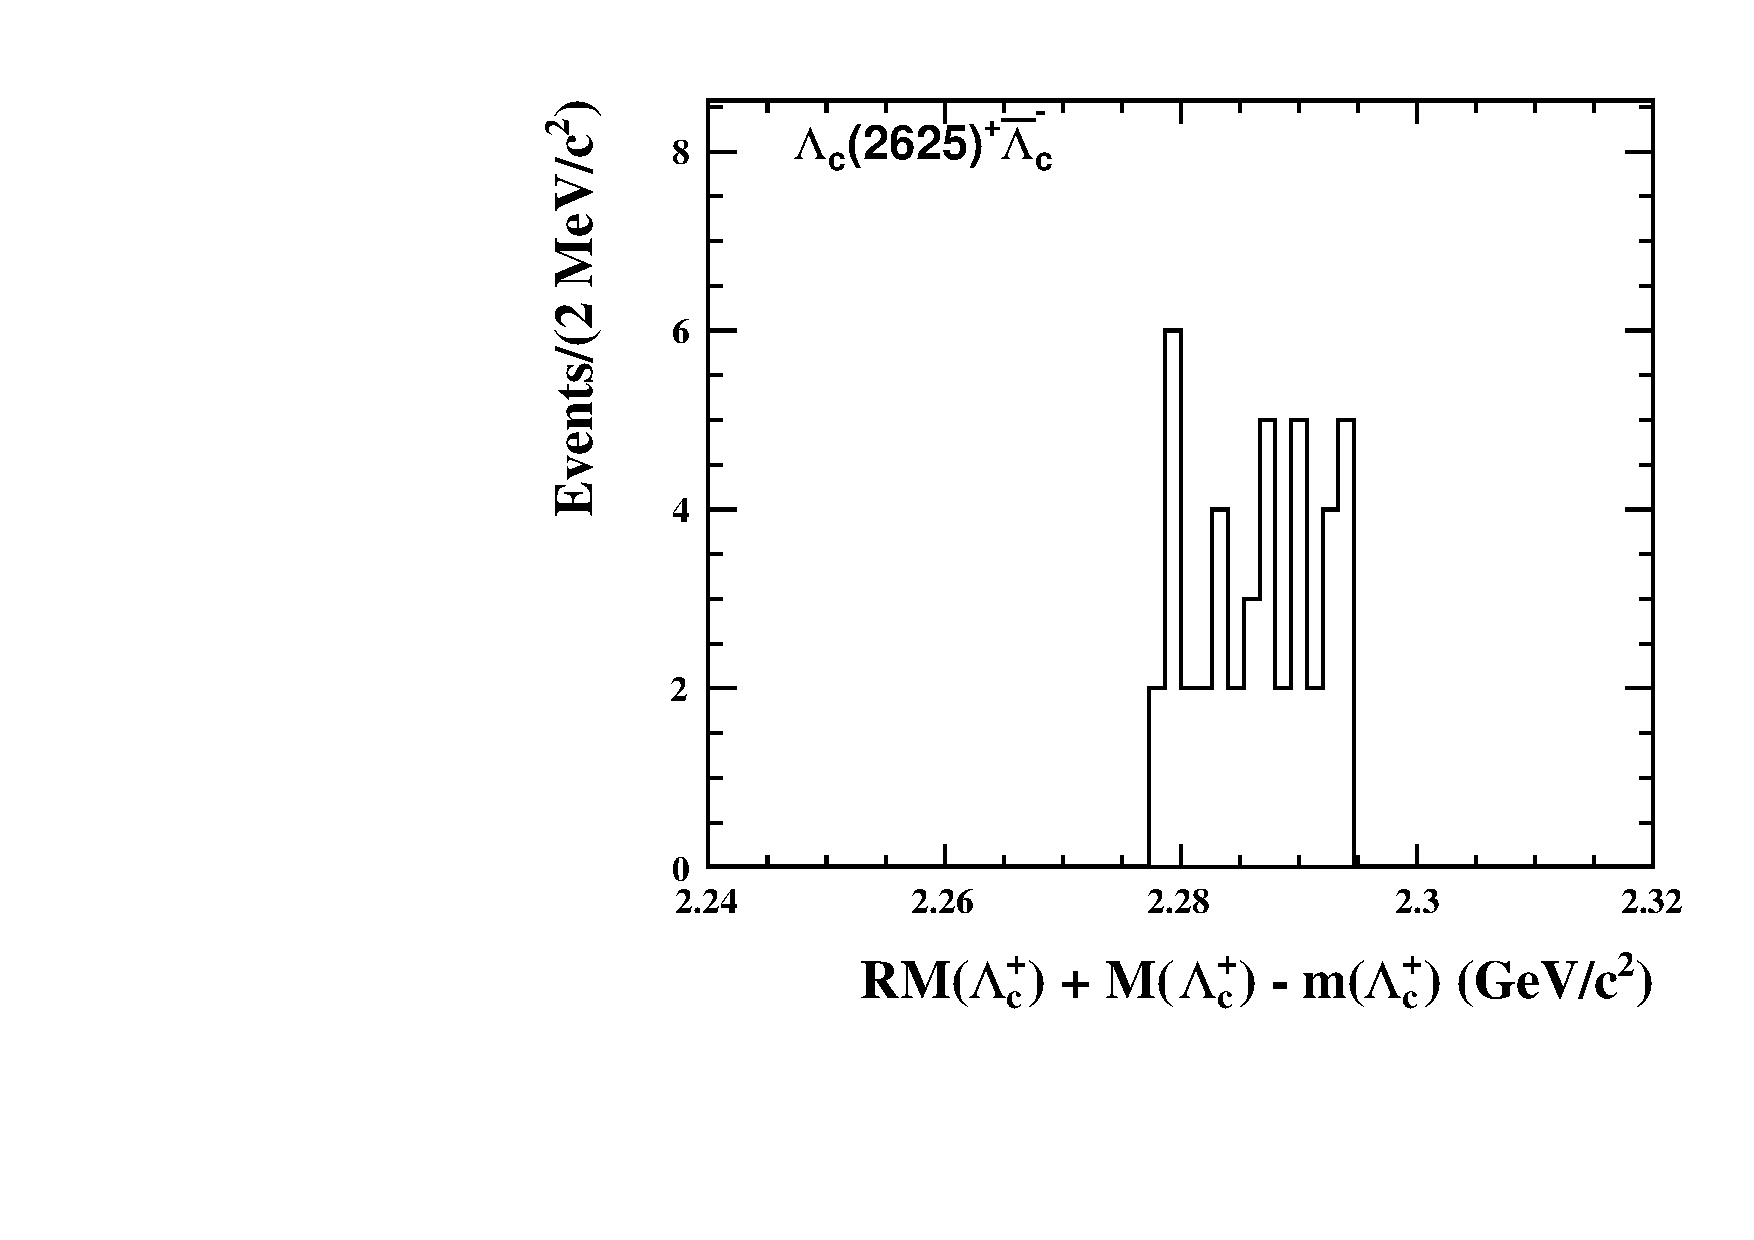
\includegraphics[width=0.45\textwidth]{figure/app_lcst/output_Lc2625_4914_rm_lmdc.pdf}
    \caption{Distribution of $RQ(\lcp)$ for  $\Lambda_c(2595)^+\lcm$ (left) and $\Lambda_c(2625)^+\lcm$ (right) at $\sqrt{s} = 4.918\gev$ in $\mbc$ signal region.}
\label{fig:mc_lcst_rm_lmdc}
\end{figure}

\begin{table}[H]
    \centering
    \caption{Total number of $\Lambda_c^{*+}\lcm$ measured by BAM-627 at $\sqrt{s}=4.918$ and 4.950$\gev/c^2$.}
    \label{tab:total_lcst}
    \begin{tabular}{c|c|c}
    \hline\hline
    $\sqrt{s}$ MeV & $e^+e^- \to \Lambda_c(2595)^+\lcm$ & $e^+e^- \to \Lambda_c(2625)^+\lcm$ \\\hline
    4918.02 & 2522.85 & 3676.29 \\\hline
    4950.93 & 3676.36 & 9434.82 \\
    \hline\hline
    \end{tabular}
\end{table}